\documentclass[10pt,a4paper]{article}
\usepackage[utf8]{inputenc}
\usepackage[T1]{fontenc}
\usepackage{geometry,graphicx,amsmath,booktabs,longtable,pdfpages,hyperref}
\geometry{margin=1.8cm}
\setlength{\parindent}{0pt}\setlength{\parskip}{0.4em}
\hypersetup{colorlinks=true,urlcolor=blue,linkcolor=blue}
\title{$\Lambda$--$^{4}\mathrm{He}$: Purity checks and Method 3/5/6 comparison}
\author{STAR analysis working report}
\date{2026-10-31 12:45 JST}
\begin{document}\maketitle
\section{Sample and calculation}
Au+Au fixed-target beam-energy label 3.85 GeV; 2021 P24iy. The beam label is not a statement about $\sqrt{s_{NN}}$. The input contains 26,955/26,994 submitted subjobs; 39 are excluded.
\textbf{SUMS:} \texttt{04BF2DAE47164B6F040E3A460E539289}. \textbf{ROOT:} \path{auau3p85_anaFemtoLambda_4He_KFParticle_04BF2DAE47164B6F040E3A460E539289_merge.root}.
Measured input/reconstructed events: 2,100,726,543 / 2,067,647,474. Existing ROOTs, PID coefficients, Maker selection and mixing are unchanged.
\begin{center}\begin{tabular}{lll}\toprule Method & Purity source & Application\\\midrule
3 & SE and ME separately & Per-CF-bin mass-fit signal $N-B$\\
5 & SE and ME separately & Coarse sliding-window purity on native counts\\
6 & ME only & Same ME purity and error on both SE and ME\\\bottomrule\end{tabular}\end{center}
Native bins: 5 MeV/$c$; CF bins: 20 MeV/$c$; Method 5/6 purity cells: 50 MeV/$c$. The sliding window uses the center and 2 neighbors on either side, clipped at the stored endpoints.
CF display: 0--0.3 GeV/$c$; normalization: 0.3--0.4 GeV/$c$. The normalization interval remains in use outside the displayed CF range. The purity plots and fit inspection include 0--0.4 GeV/$c$.
The mass model is Gaussian plus quadratic background for the \emph{$\Lambda$ invariant mass}. This does not modify the accepted helium dE/dx PID model. No mass-model shape or acceptance threshold is relaxed to obtain successful fits.
\subsection*{Centrality selections}
2 selections: 20-80\%, 0-20\%.
3 selections: 0-10\%, 10-20\%, 20-60\%.
\clearpage\section{Mass-fit reliability checks}
The table inspects fit cells with centers in the stated inspection range, including normalization. Accepted means the full-window background is physically usable under the numerical checks; it does not establish model adequacy. A boundary warning is recorded separately. The minimum and median observation counts refer to the entire fitted mass projection, not only its signal window or central purity cell.
{\scriptsize\setlength{\tabcolsep}{3pt}\begin{longtable}{llcrrrrrr}\toprule Centrality & Method & Side & Accepted/total & Boundary & Min obs. & Median obs. & Median $\chi^2/\nu$ & Max $\chi^2/\nu$\\\midrule\endhead
20-80\% & 3 & SE & 18/20 & 2 & 3 & 1539 & 1.092 & 1.83\\
20-80\% & 3 & ME & 20/20 & 1 & 139 & 6.384e+04 & 4.993 & 21.04\\
20-80\% & 5 & SE & 8/8 & 0 & 1780 & 2.178e+04 & 3.536 & 9.496\\
20-80\% & 5 & ME & 7/8 & 0 & 6.925e+04 & 8.977e+05 & 60.17 & 557.5\\
0-20\% & 3 & SE & 19/20 & 1 & 22 & 8464 & 2.333 & 5.909\\
0-20\% & 3 & ME & 20/20 & 0 & 937 & 3.085e+05 & 33.13 & 151.2\\
0-20\% & 5 & SE & 8/8 & 0 & 1.163e+04 & 1.194e+05 & 16.7 & 50.55\\
0-20\% & 5 & ME & 8/8 & 0 & 4.167e+05 & 4.366e+06 & 504.5 & 1770\\
0-10\% & 3 & SE & 19/20 & 0 & 15 & 6600 & 2.261 & 4.876\\
0-10\% & 3 & ME & 20/20 & 0 & 781 & 2.422e+05 & 27.73 & 123.1\\
0-10\% & 5 & SE & 8/8 & 0 & 9224 & 9.261e+04 & 13.45 & 40.3\\
0-10\% & 5 & ME & 8/8 & 0 & 3.328e+05 & 3.403e+06 & 421.2 & 1435\\
10-20\% & 3 & SE & 18/20 & 1 & 7 & 1865 & 1.263 & 2.705\\
10-20\% & 3 & ME & 20/20 & 1 & 156 & 6.633e+04 & 6.832 & 29.49\\
10-20\% & 5 & SE & 8/8 & 0 & 2409 & 2.683e+04 & 4.593 & 11.38\\
10-20\% & 5 & ME & 8/8 & 0 & 8.385e+04 & 9.631e+05 & 88.42 & 341.3\\
20-60\% & 3 & SE & 18/20 & 2 & 3 & 1536 & 1.092 & 1.814\\
20-60\% & 3 & ME & 20/20 & 1 & 138 & 6.304e+04 & 5.012 & 22.21\\
20-60\% & 5 & SE & 8/8 & 0 & 1769 & 2.171e+04 & 4.085 & 9.539\\
20-60\% & 5 & ME & 8/8 & 0 & 6.859e+04 & 8.878e+05 & 60.15 & 231.5\\
\bottomrule\end{longtable}}
Sparse Method 3 SE spectra can have poorly determined backgrounds even when the minimizer returns status zero. For Method 5, a low-count central cell is fitted using a broader sliding projection: the central-cell count alone is not the fit sample size. Large $\chi^2/\nu$ or small fit probabilities remain a separate problem at high statistics. The atlas retains all projections, including failures and boundary solutions, with model curves, pulls and normalized SE/ME mass shapes.
Purity differences alone do not identify the cause. The figures permit checking low statistics, nonphysical fitted background, covariance failure, and persistent mass-shape/model discrepancy separately. No numerical goodness threshold is silently used as a new selection cut.
\subsection*{Representative low-$k^*$ and normalization fits}
{\scriptsize\begin{tabular}{llcrrrr}\toprule Centrality & Method & Cell & $k^*$ & $P_{\rm SE}$ & $P_{\rm ME}$ & SE/ME fitted observations\\\midrule
20-80\% & 3 & 1 & 0.01 & NA & $0.72983\pm0.0583$ & 3 / 139\\
20-80\% & 3 & 6 & 0.11 & $0.86725\pm0.0177$ & $0.82303\pm0.00272$ & 401 / 1.446e+04\\
20-80\% & 3 & 16 & 0.31 & $0.93741\pm0.00346$ & $0.90199\pm0.000617$ & 3702 / 1.532e+05\\
0-20\% & 3 & 1 & 0.01 & NA & $0.92557\pm0.00738$ & 22 / 937\\
0-20\% & 3 & 6 & 0.11 & $0.9472\pm0.00339$ & $0.92065\pm0.000525$ & 2448 / 8.98e+04\\
0-20\% & 3 & 16 & 0.31 & $0.95303\pm0.000839$ & $0.94852\pm0.00015$ & 1.995e+04 / 7.295e+05\\
20-80\% & 5 & 1 & 0.025 & $0.8994\pm0.00665$ & $0.82777\pm0.00198$ & 1780 / 6.925e+04\\
20-80\% & 5 & 3 & 0.125 & $0.90683\pm0.00278$ & $0.86104\pm0.000484$ & 9694 / 3.93e+05\\
20-80\% & 5 & 7 & 0.325 & $0.93502\pm0.000951$ & NA & 4.918e+04 / 2.035e+06\\
0-20\% & 5 & 1 & 0.025 & $0.91635\pm0.00157$ & $0.92086\pm0.000249$ & 1.163e+04 / 4.167e+05\\
0-20\% & 5 & 3 & 0.125 & $0.93271\pm0.000594$ & $0.93292\pm0.000179$ & 5.491e+04 / 1.985e+06\\
0-20\% & 5 & 7 & 0.325 & $0.95245\pm0.000234$ & $0.95061\pm3.95e-05$ & 2.706e+05 / 1.001e+07\\
\bottomrule\end{tabular}}
\clearpage\section{Meaning and uncertainty of Method 6}
SE and ME purity equality is an assumption to test, not a requirement. Let the mixed-event signal/background be $S_m,B_m$, and let the same-event components be proportional to $C_sS_m,C_bB_m$ with a common scale. Then
\[P_{\rm SE}=\frac{C_sP_{\rm ME}}{C_sP_{\rm ME}+C_b(1-P_{\rm ME})}.\]
Thus different signal and background correlations can produce different purities even with arbitrarily large statistics. Method 6 is the requested common-ME-purity transfer comparison; the agreement imposed by its construction is not evidence that the transfer is unbiased.
For each native cell, $A=P_{\rm ME}N_{\rm SE}$ and $B=P_{\rm ME}N_{\rm ME}$ use the same random purity estimate, including the same ME-derived error. For a ratio wholly inside one purity cell, $A/B=N_{\rm SE}/N_{\rm ME}$ and the local purity uncertainty cancels. An output bin crossing two purity cells, and the weighted normalization integrals, can retain purity dependence. Purity is applied before rebinning; assigning one purity using the output-bin center would give a different answer.
The calculation retains the shared-purity SE--ME covariance, normalization covariance, and covariance caused by reuse of observed counts in overlapping purity windows. The saved full covariance matrices should be used instead of treating plotted CF points as independent. Errors are first-order estimates using the supplied histogram variances and background-fit covariance.
\textbf{Not included:} background-fit/count covariance, cross-fit background-parameter covariance, missing event/track/mixed-pair reuse correlations, cross-method covariance, and the model/transfer systematic uncertainty of applying ME purity to SE. Near zero observed counts, plug-in Poisson variances and Gaussian error propagation have limited coverage. A smaller Method 6 error bar does not establish that its transfer assumption is correct. No independent-error significance is assigned to differences between methods.
\subsection*{Missing fits and normalization}
All normalization bins require usable positive SE and ME signal yields. If any contributing fit is unavailable, the entire group CF is NA; no smaller normalization interval is substituted. A failed ME purity masks both Method 6 sides. Sharing ME purity cannot repair a failed ME normalization fit. Missing values are not physical zero measurements.
\clearpage\section{CF comparison and figure guide}
The integrated CF below is the ratio of summed yields over 0--0.2 GeV/$c$, multiplied by the separately evaluated normalization. It is not an arithmetic mean of plotted CF points. The numbers use the present shared-input covariance propagation; their errors should not be read as independent errors across methods.
\begin{center}\begin{tabular}{lrrr}\toprule Centrality & Method 3 & Method 5 & Method 6\\\midrule
20-80\% & NA & NA & NA\\
0-20\% & NA & $1.0241\pm0.00879$ & $1.0262\pm0.00855$\\
0-10\% & NA & $1.0246\pm0.00984$ & $1.0276\pm0.00959$\\
10-20\% & NA & $1.0446\pm0.02$ & $1.0305\pm0.0191$\\
20-60\% & NA & $1.1015\pm0.0266$ & $1.0774\pm0.025$\\
\bottomrule\end{tabular}\end{center}
\subsection*{Groups unavailable because of normalization fits}
{\small\begin{itemize}
\item 20-80\% / Method 5: ME bin 16: invalid contributing mass fit; ME bin 17: invalid contributing mass fit; ME bin 18: invalid contributing mass fit
\item 20-80\% / Method 6: SE bin 16: invalid contributing mass fit; ME bin 16: invalid contributing mass fit; SE bin 17: invalid contributing mass fit; ME bin 17: invalid contributing mass fit; SE bin 18: invalid contributing mass fit; ME bin 18: invalid contributing mass fit
\end{itemize}}
\subsection*{Pages that follow}
The next two original pages compare CFs for the two-way and three-way centrality selections; the next two compare SE/ME purities over the inspection range. Method 6 uses identical ME purity/error on both sides by construction. The final representative pages show the configured cells for both groups of the two-way selection, first Method 3 and then Method 5. Full atlases remain separate so that every inspected fit is available without expanding this report to hundreds of pages.
\path{methods_comparison.json} contains CF values, covariance, purity and masks; \path{purity_fit_review.json} contains the fitted mass projections and fit parameters; \path{report_metadata.json} records dependencies and hashes. The comparison does not refit or choose final interaction parameters.
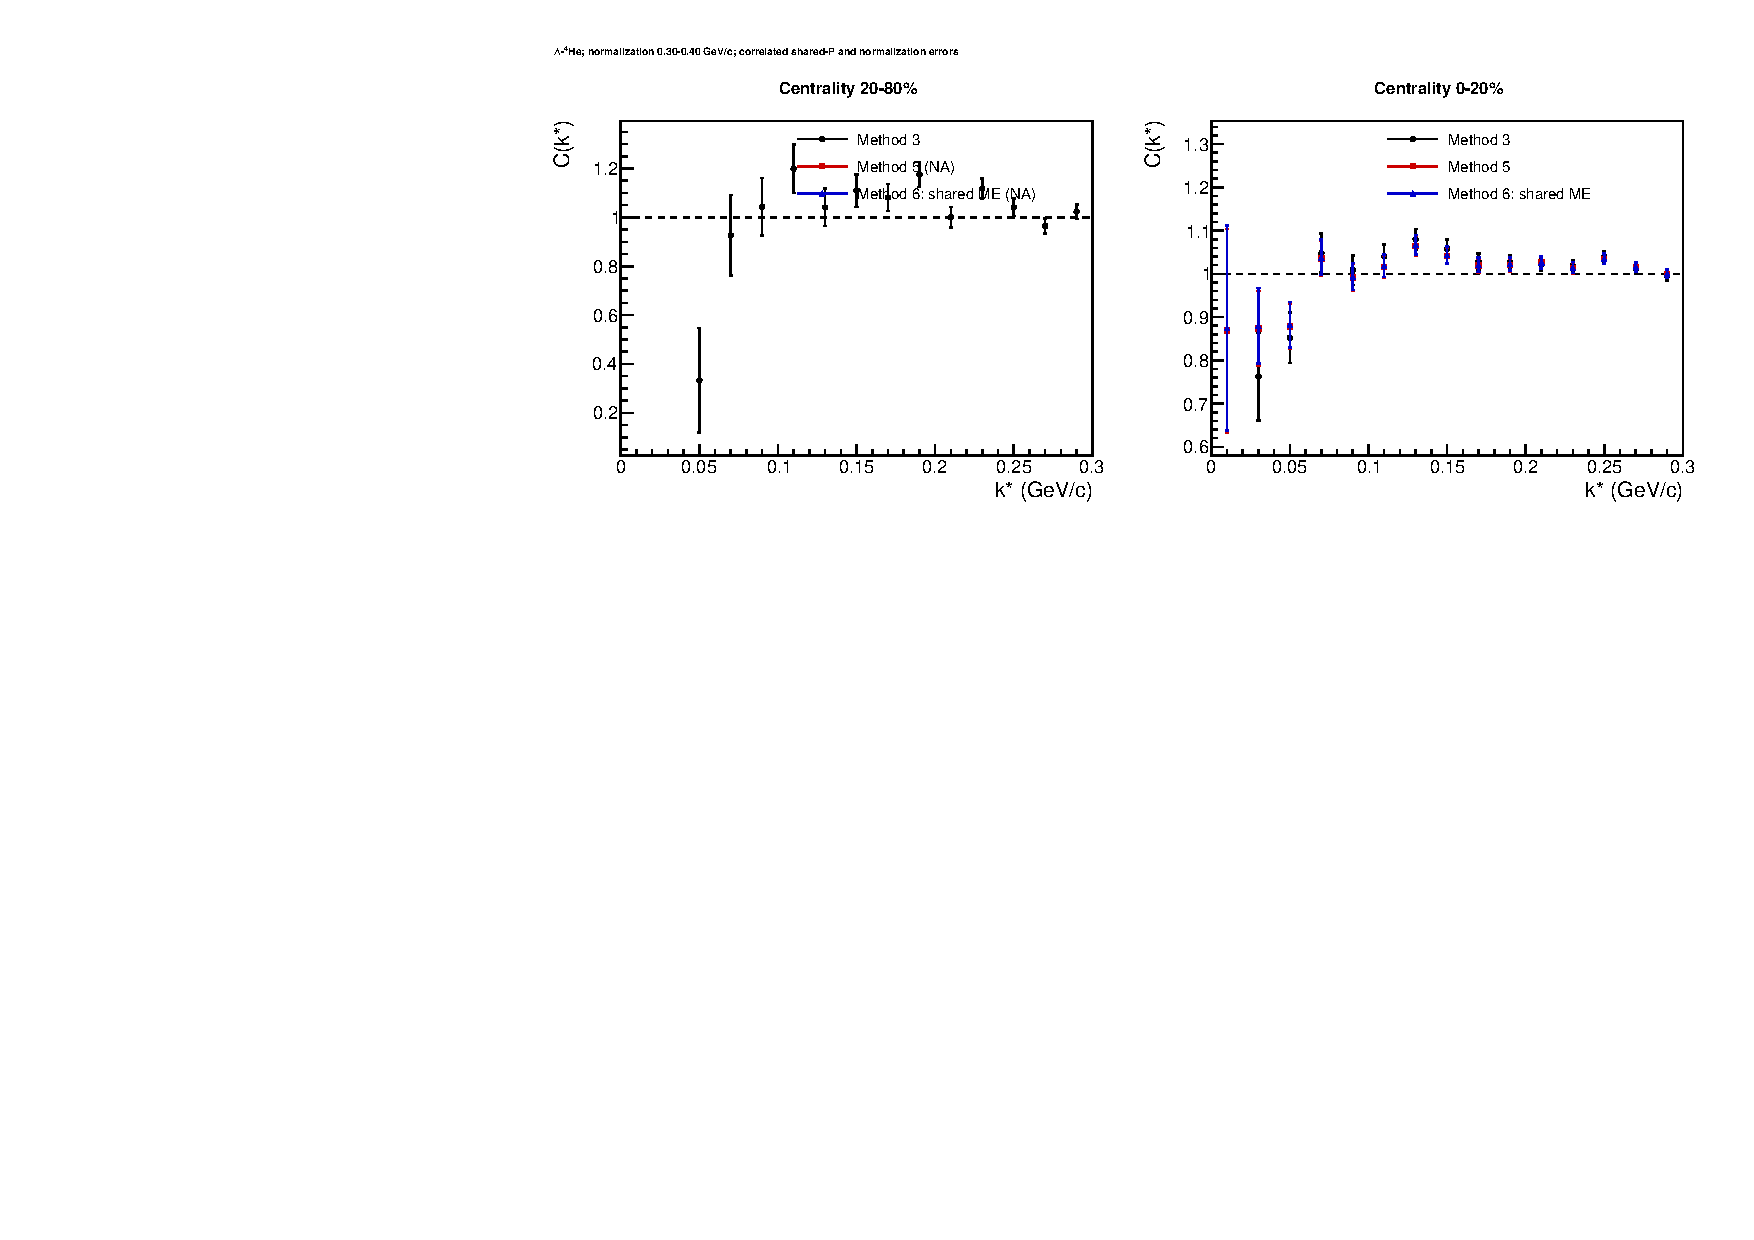
\includepdf[pages={-},fitpaper=true,pagecommand={}]{cf_methods_3_5_6.pdf}
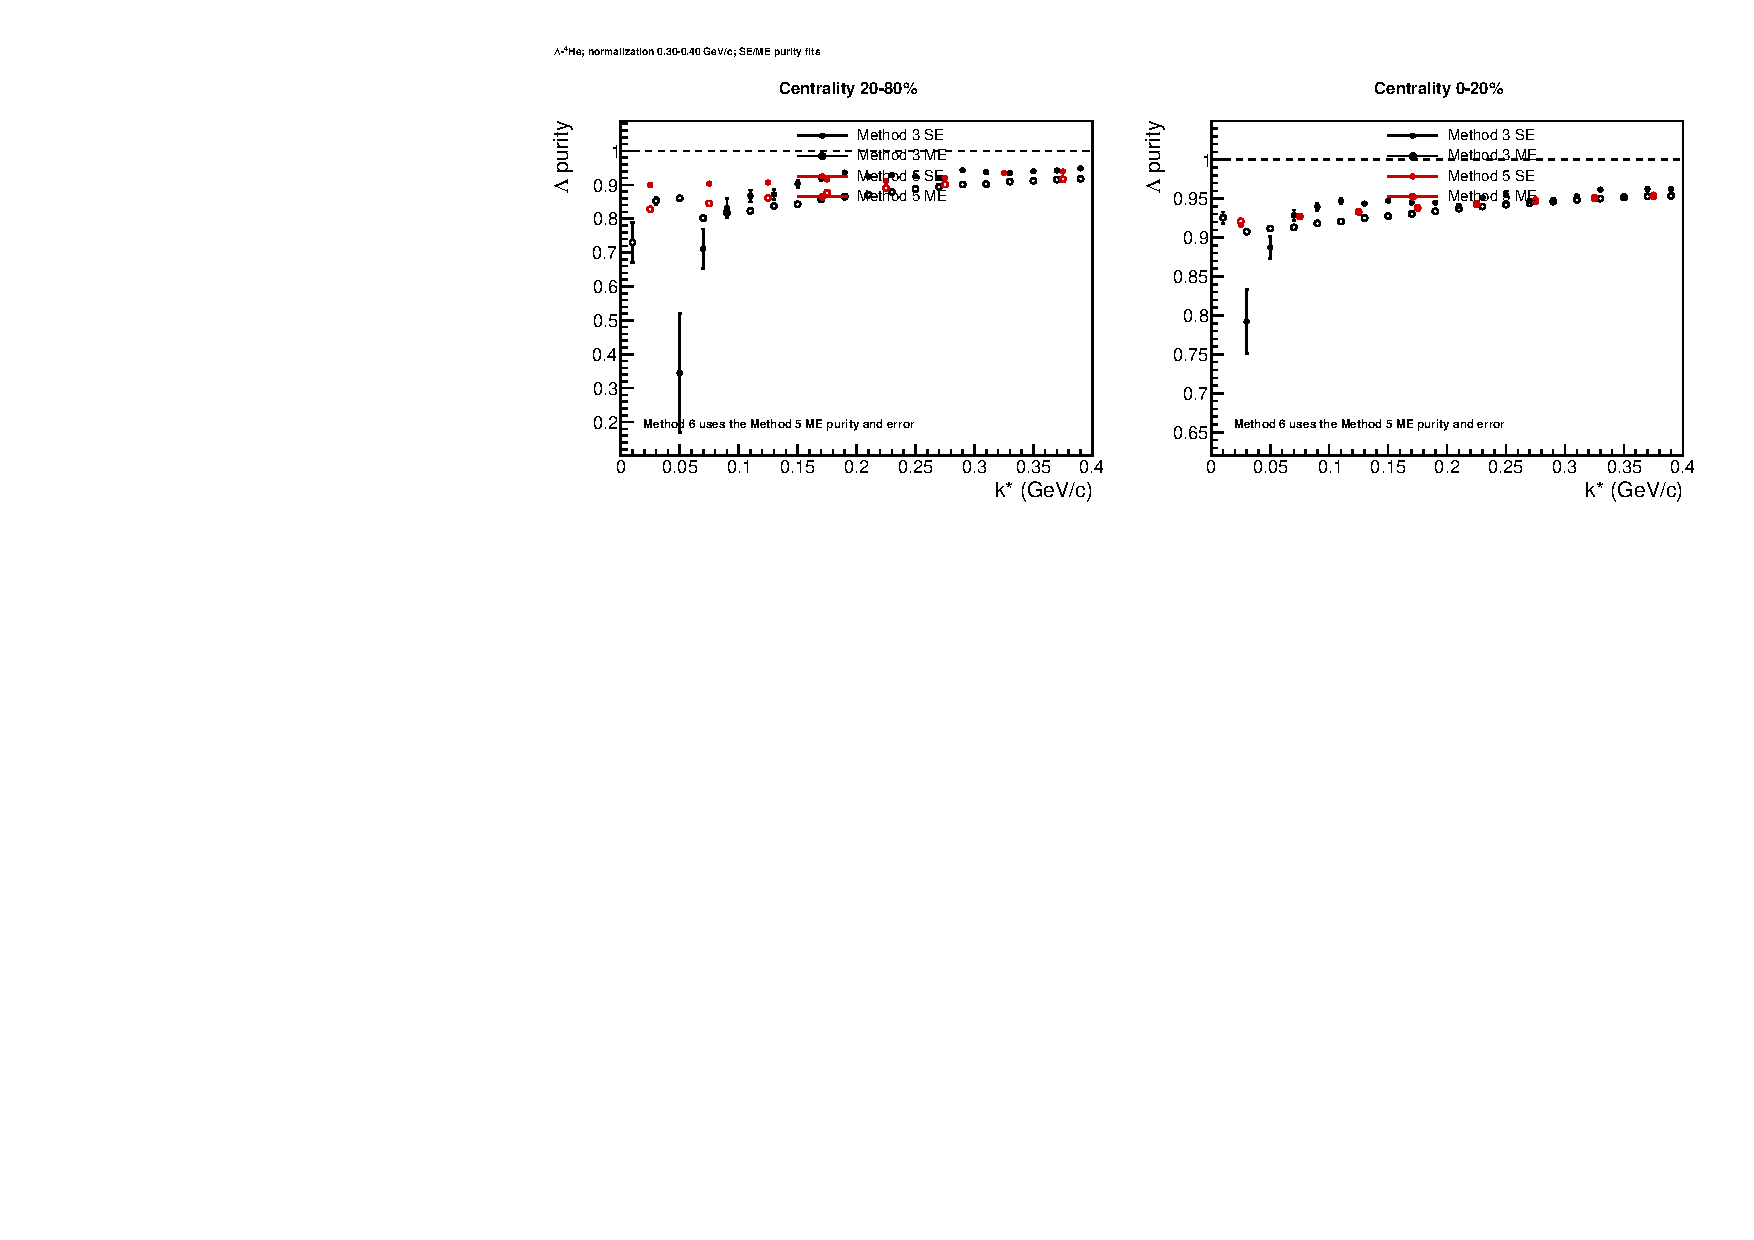
\includepdf[pages={-},fitpaper=true,pagecommand={}]{purity_se_me.pdf}
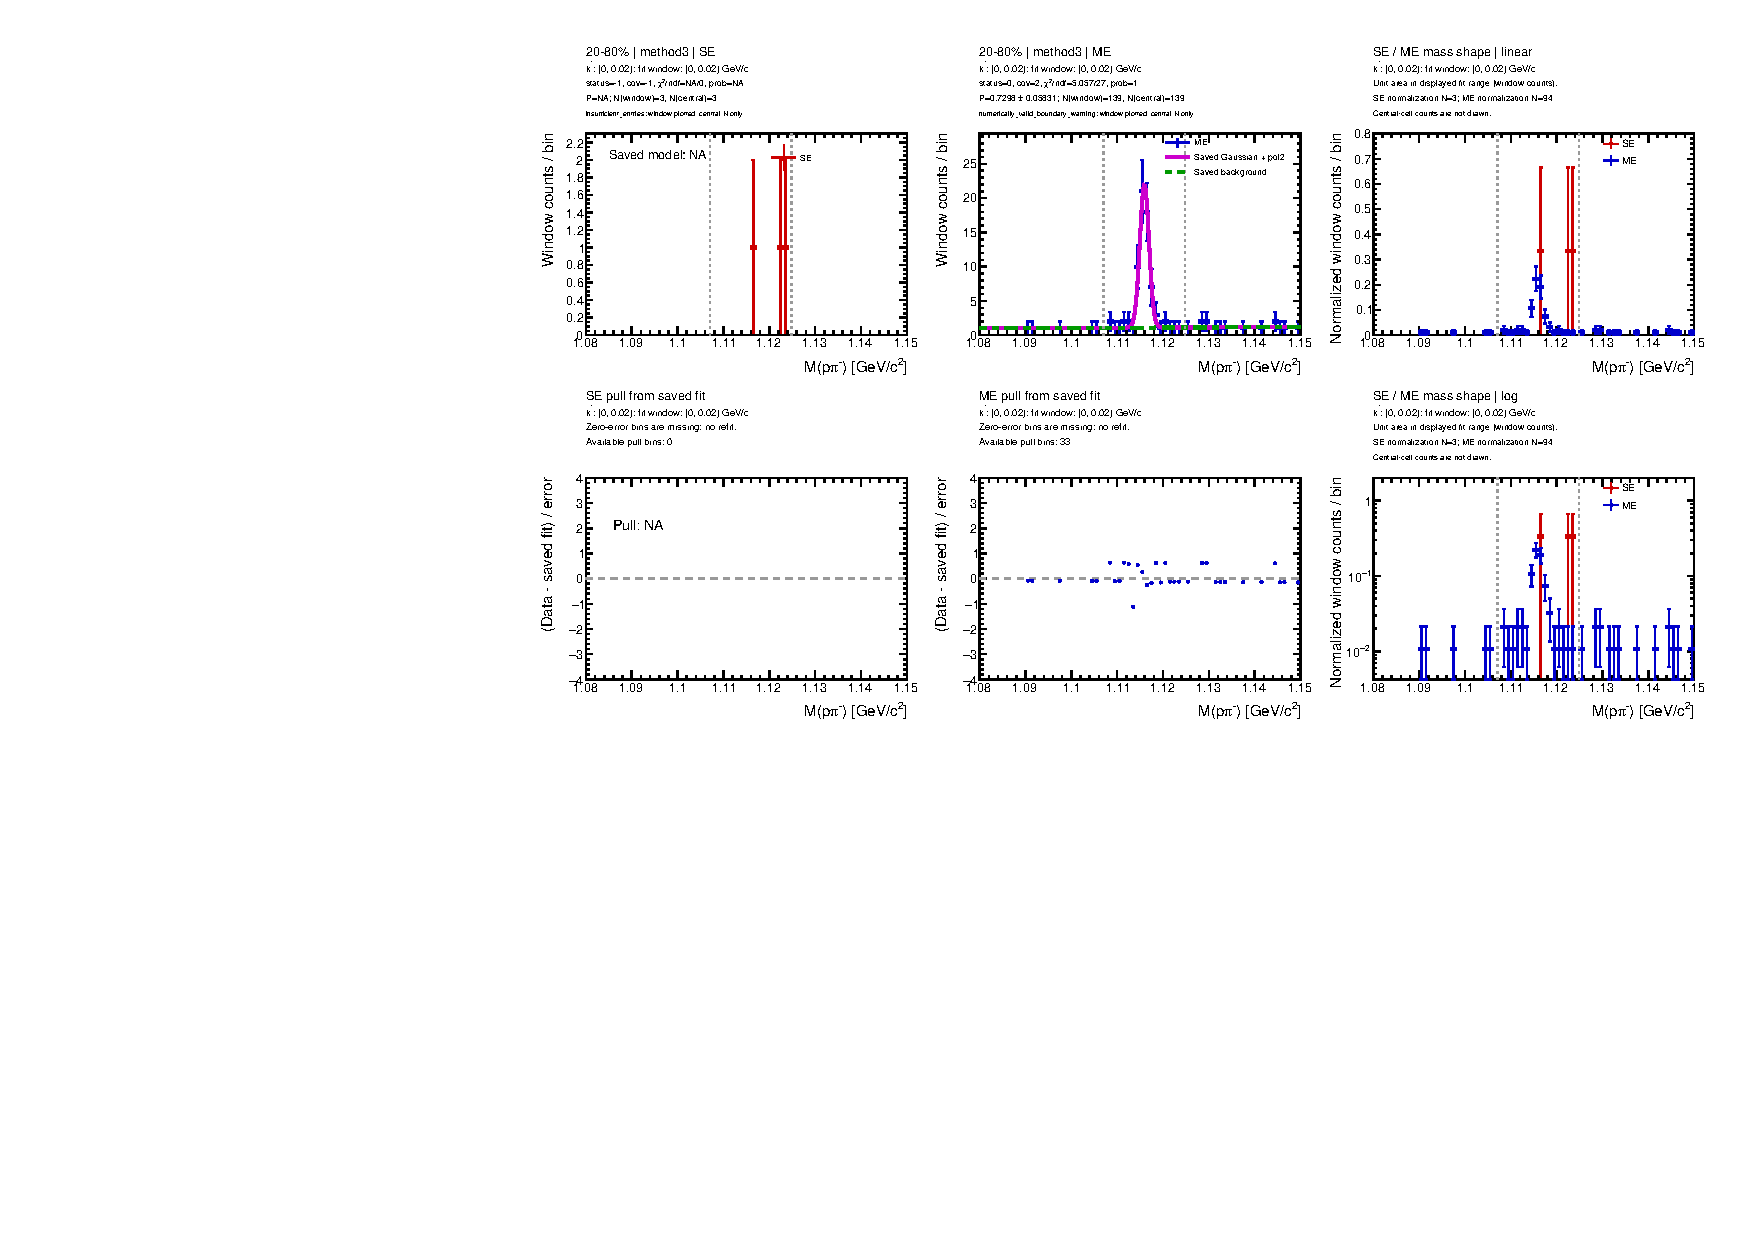
\includepdf[pages={1},fitpaper=true,pagecommand={}]{fit_method3_cent20_80_001.pdf}
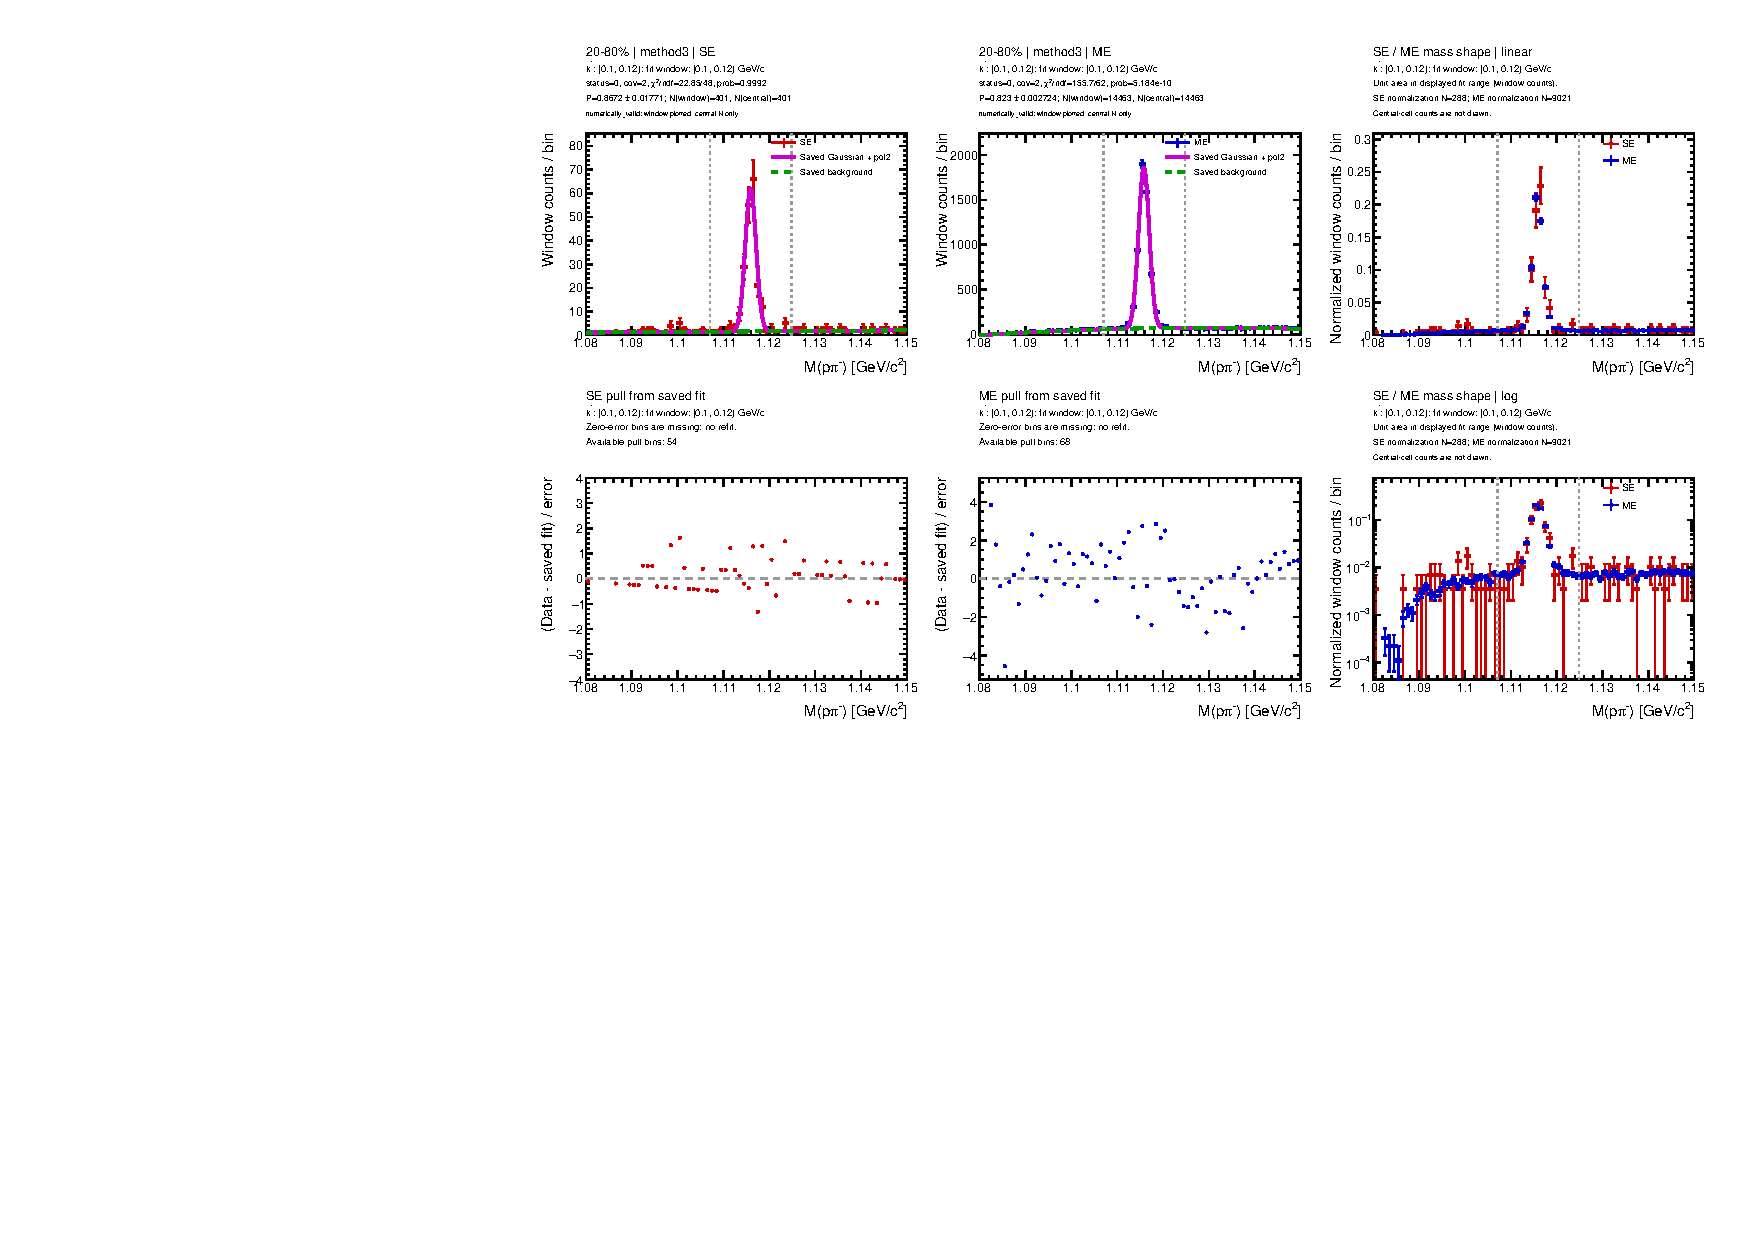
\includepdf[pages={1},fitpaper=true,pagecommand={}]{fit_method3_cent20_80_006.pdf}
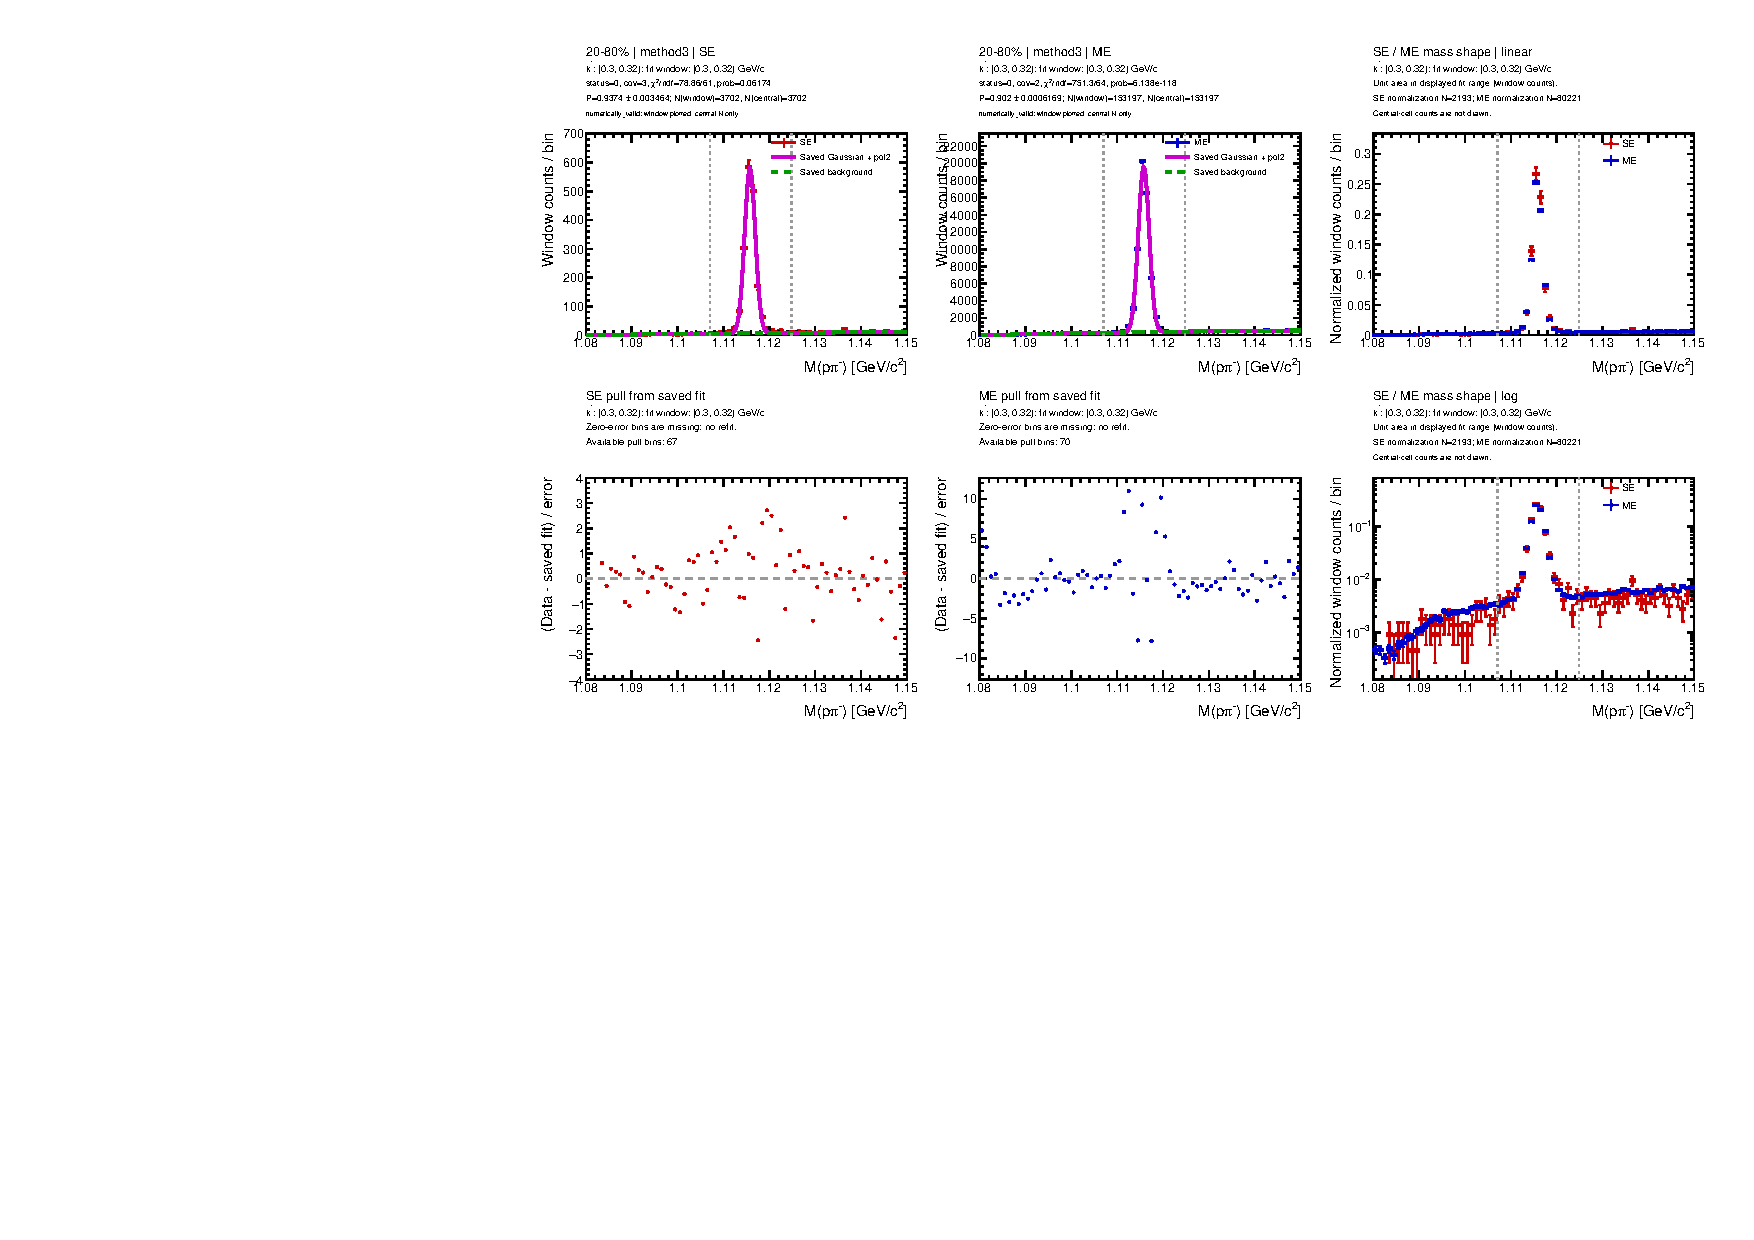
\includepdf[pages={1},fitpaper=true,pagecommand={}]{fit_method3_cent20_80_016.pdf}
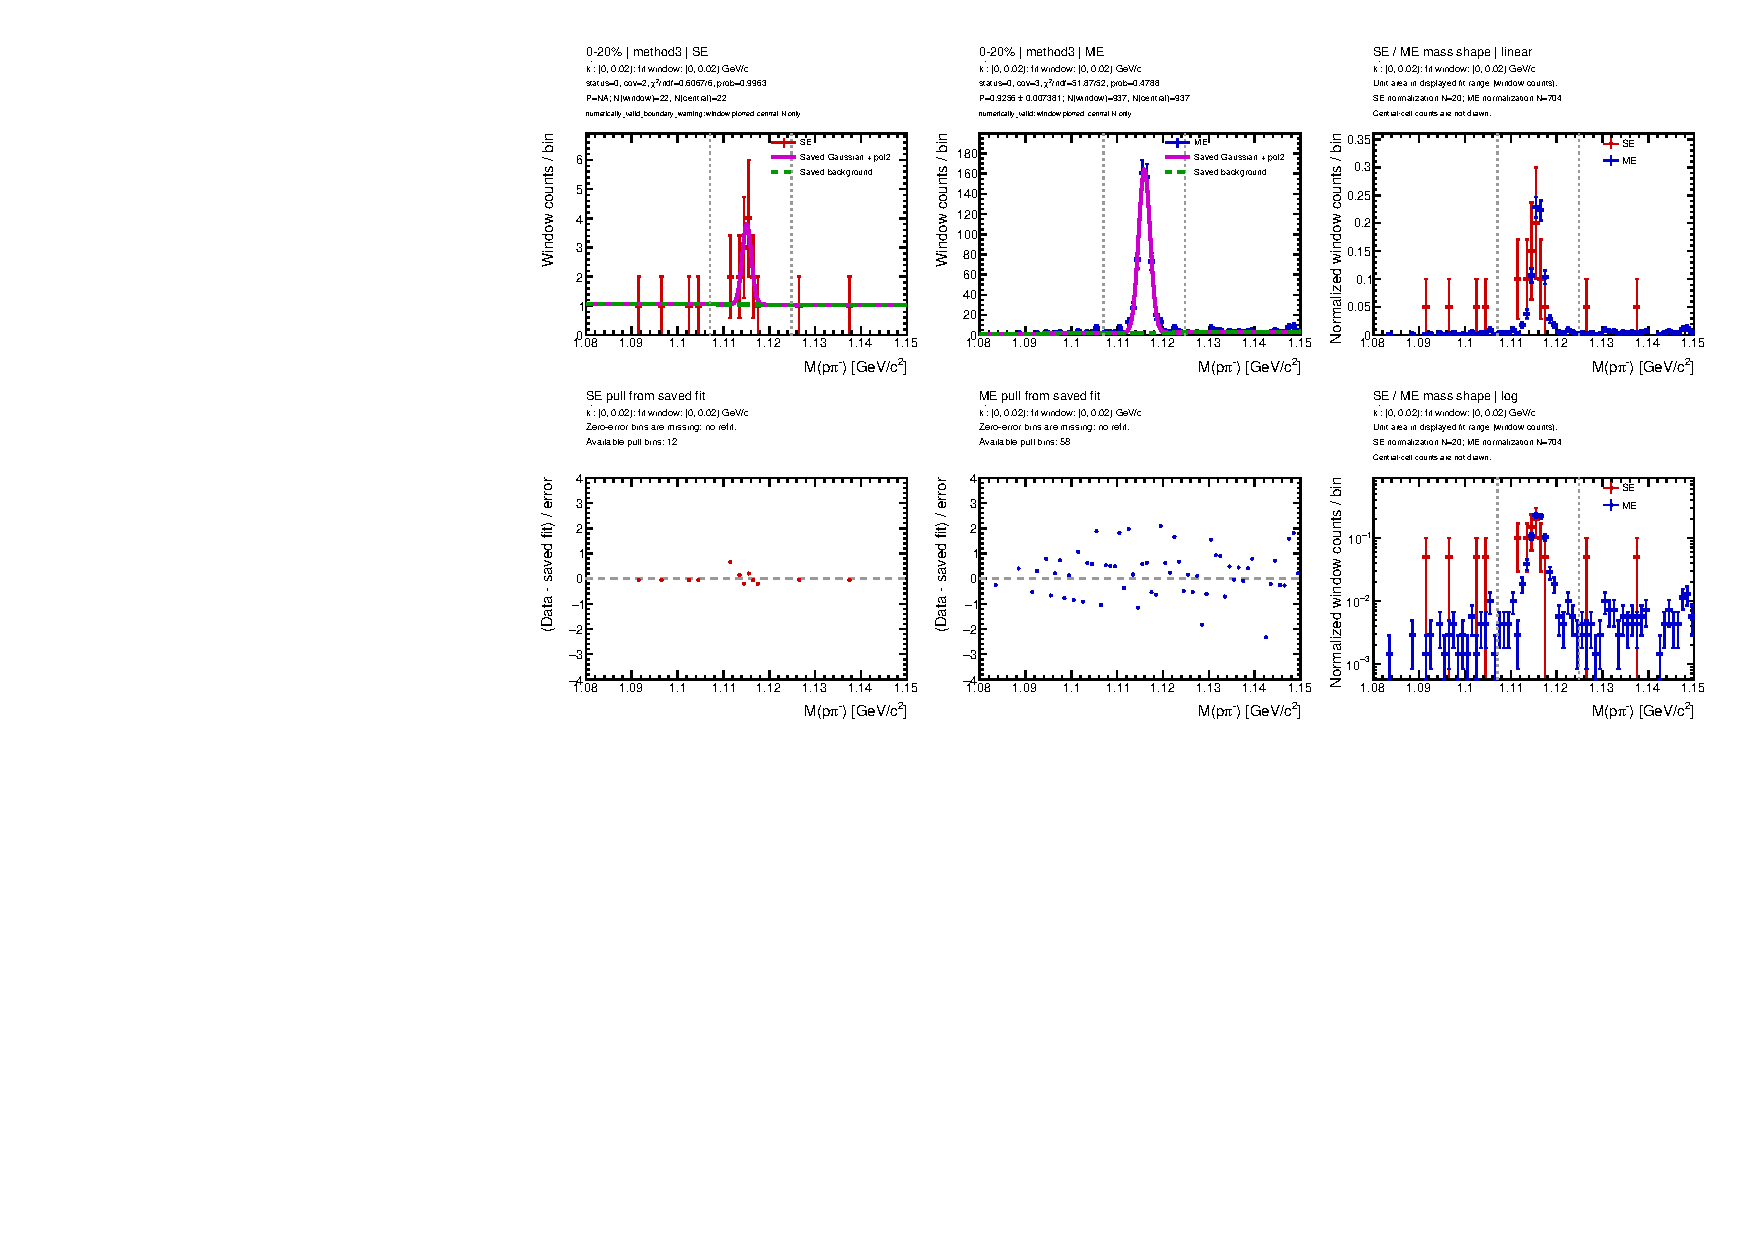
\includepdf[pages={1},fitpaper=true,pagecommand={}]{fit_method3_cent0_20_001.pdf}
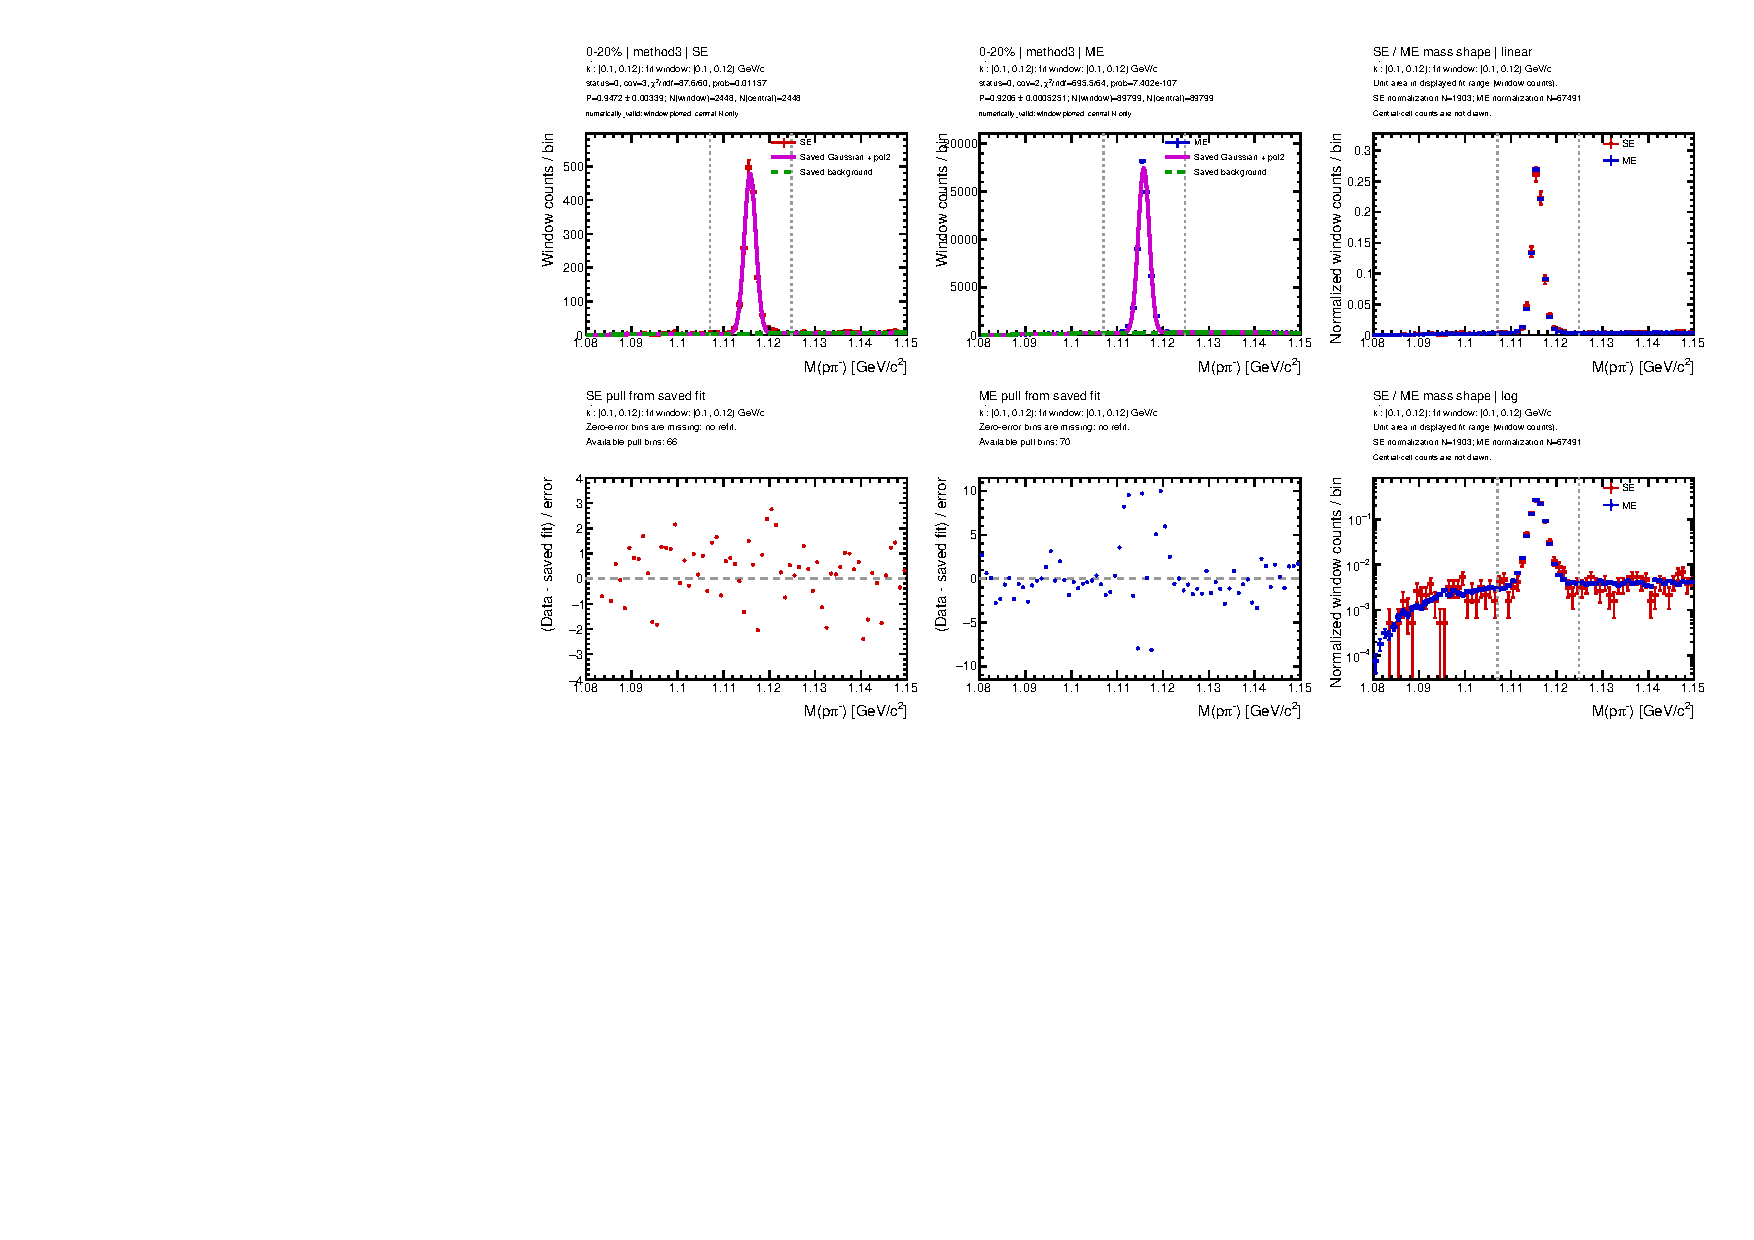
\includepdf[pages={1},fitpaper=true,pagecommand={}]{fit_method3_cent0_20_006.pdf}
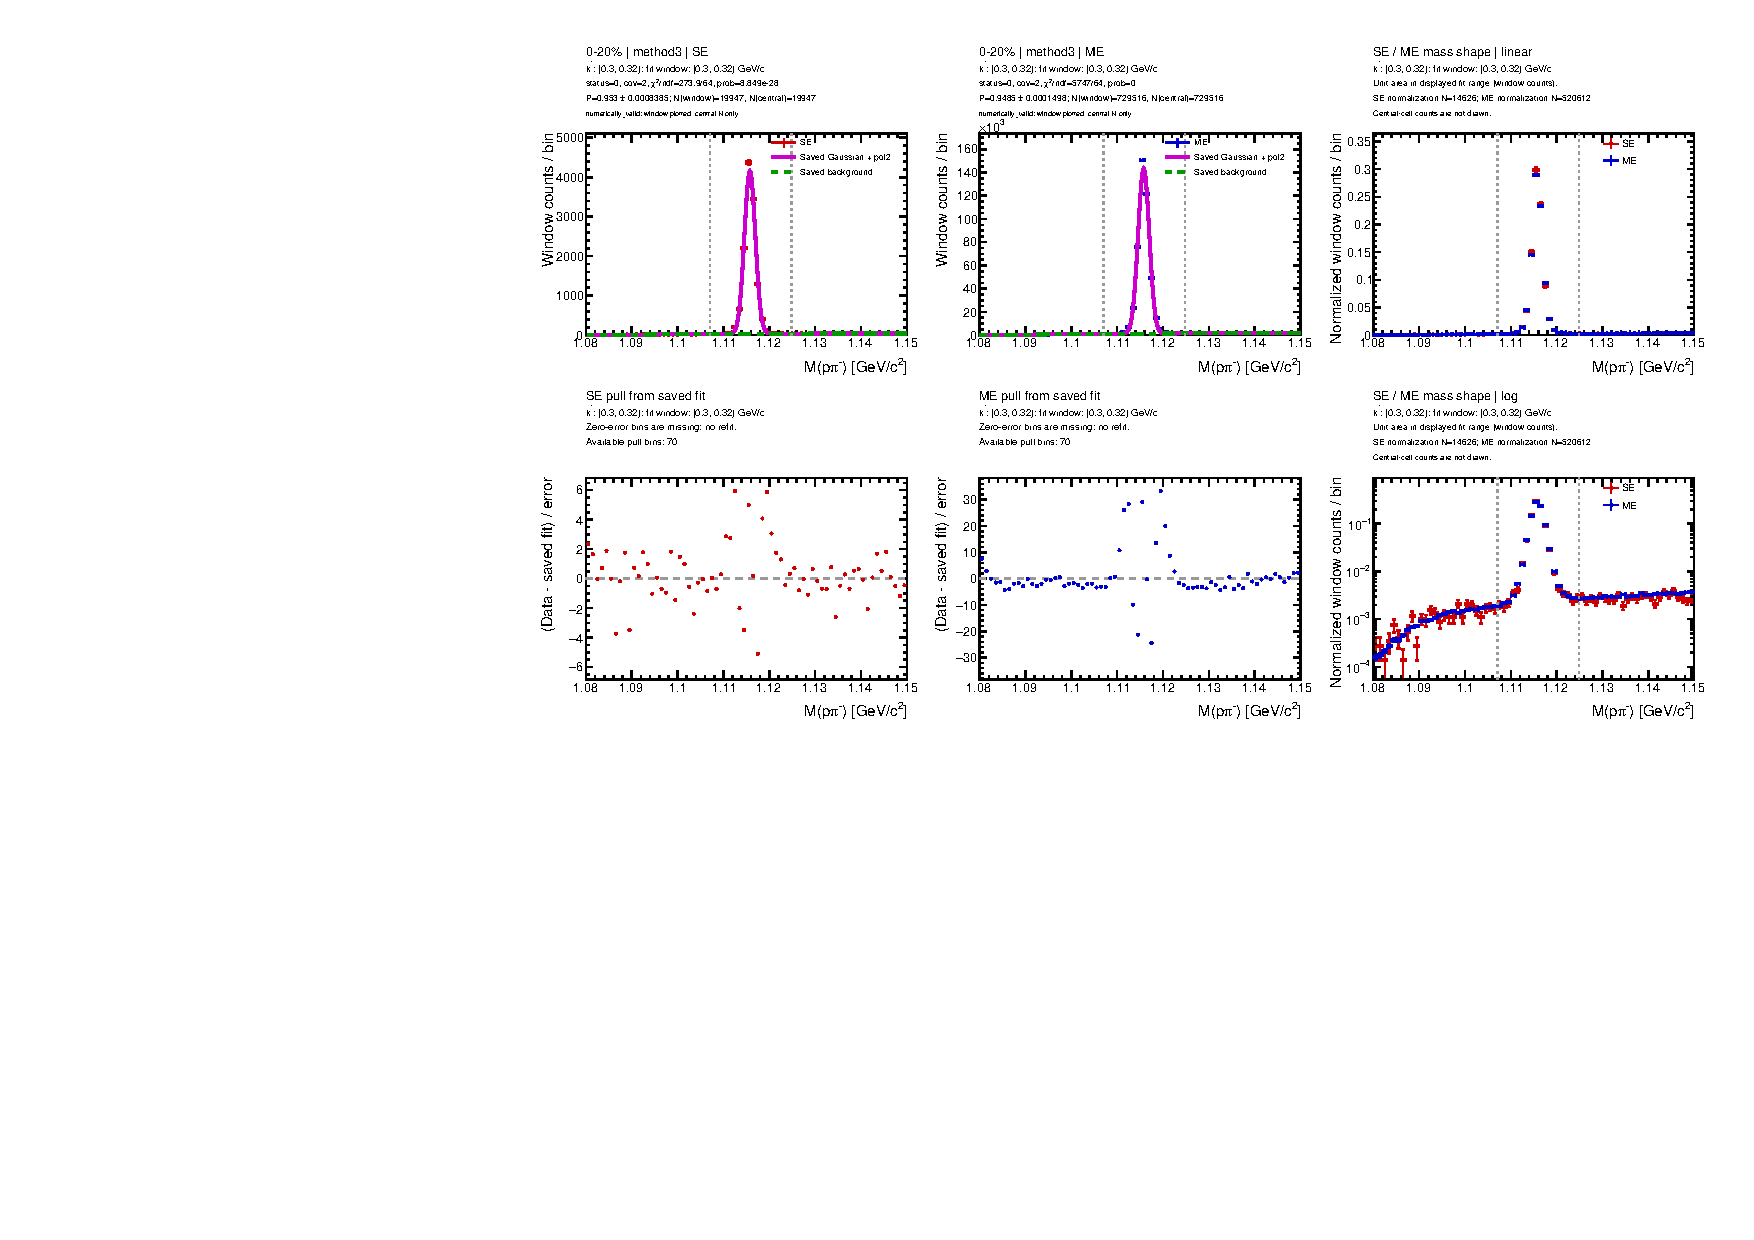
\includepdf[pages={1},fitpaper=true,pagecommand={}]{fit_method3_cent0_20_016.pdf}
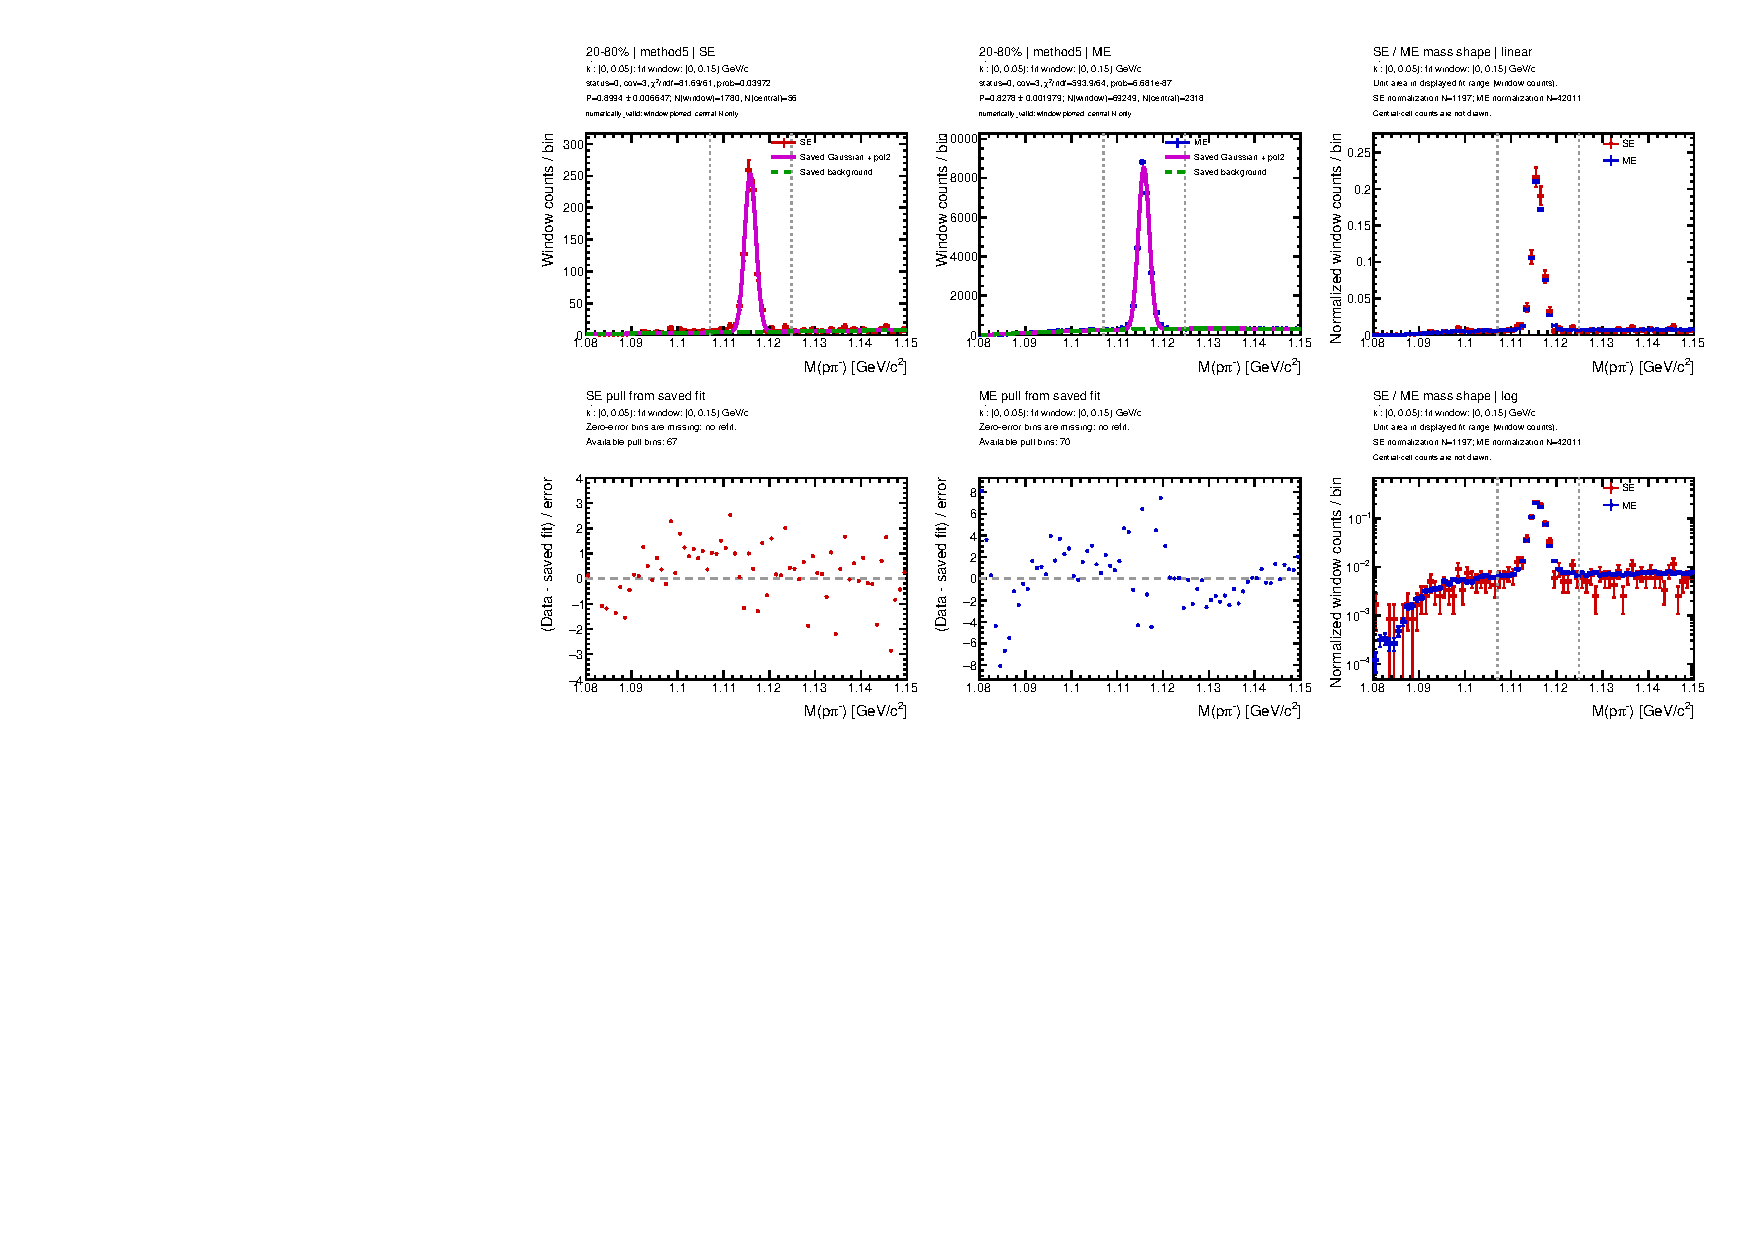
\includepdf[pages={1},fitpaper=true,pagecommand={}]{fit_method5_cent20_80_001.pdf}
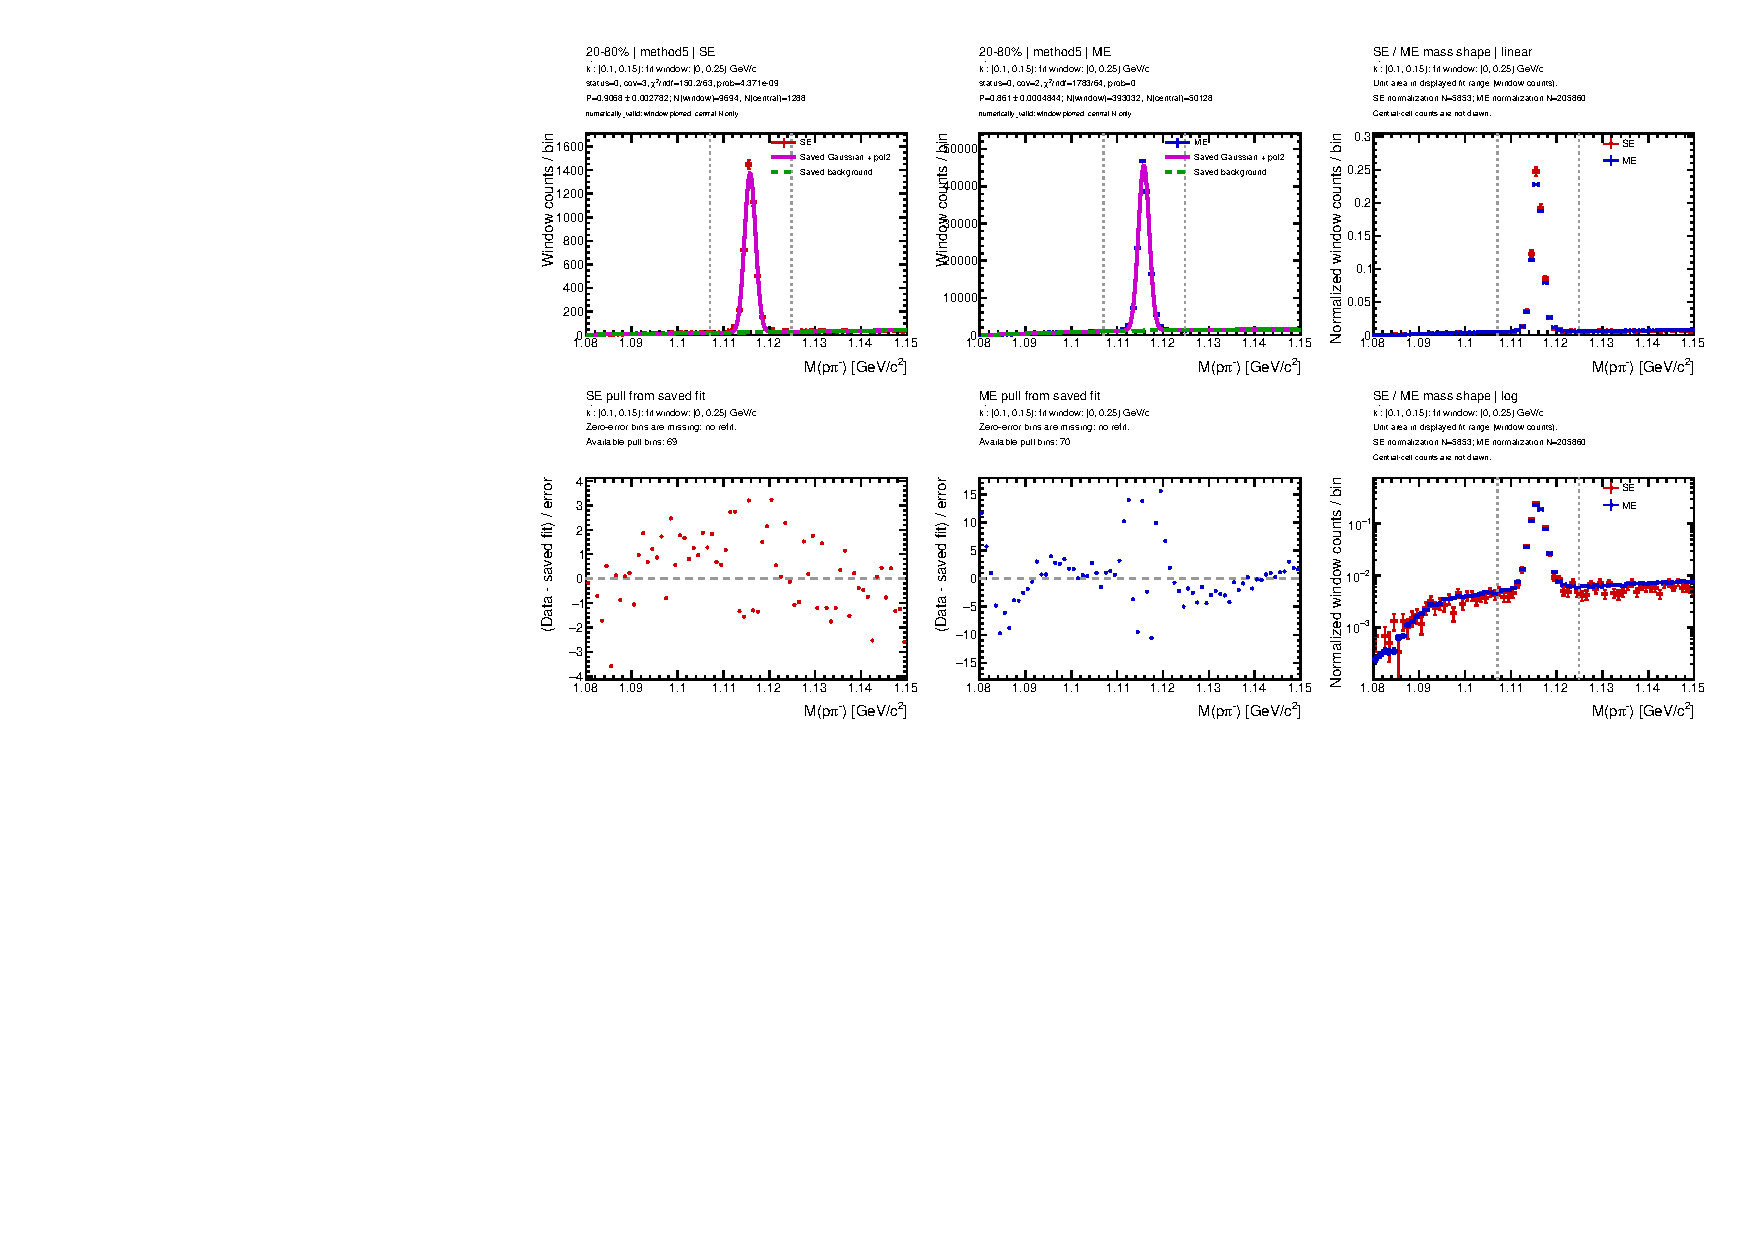
\includepdf[pages={1},fitpaper=true,pagecommand={}]{fit_method5_cent20_80_003.pdf}
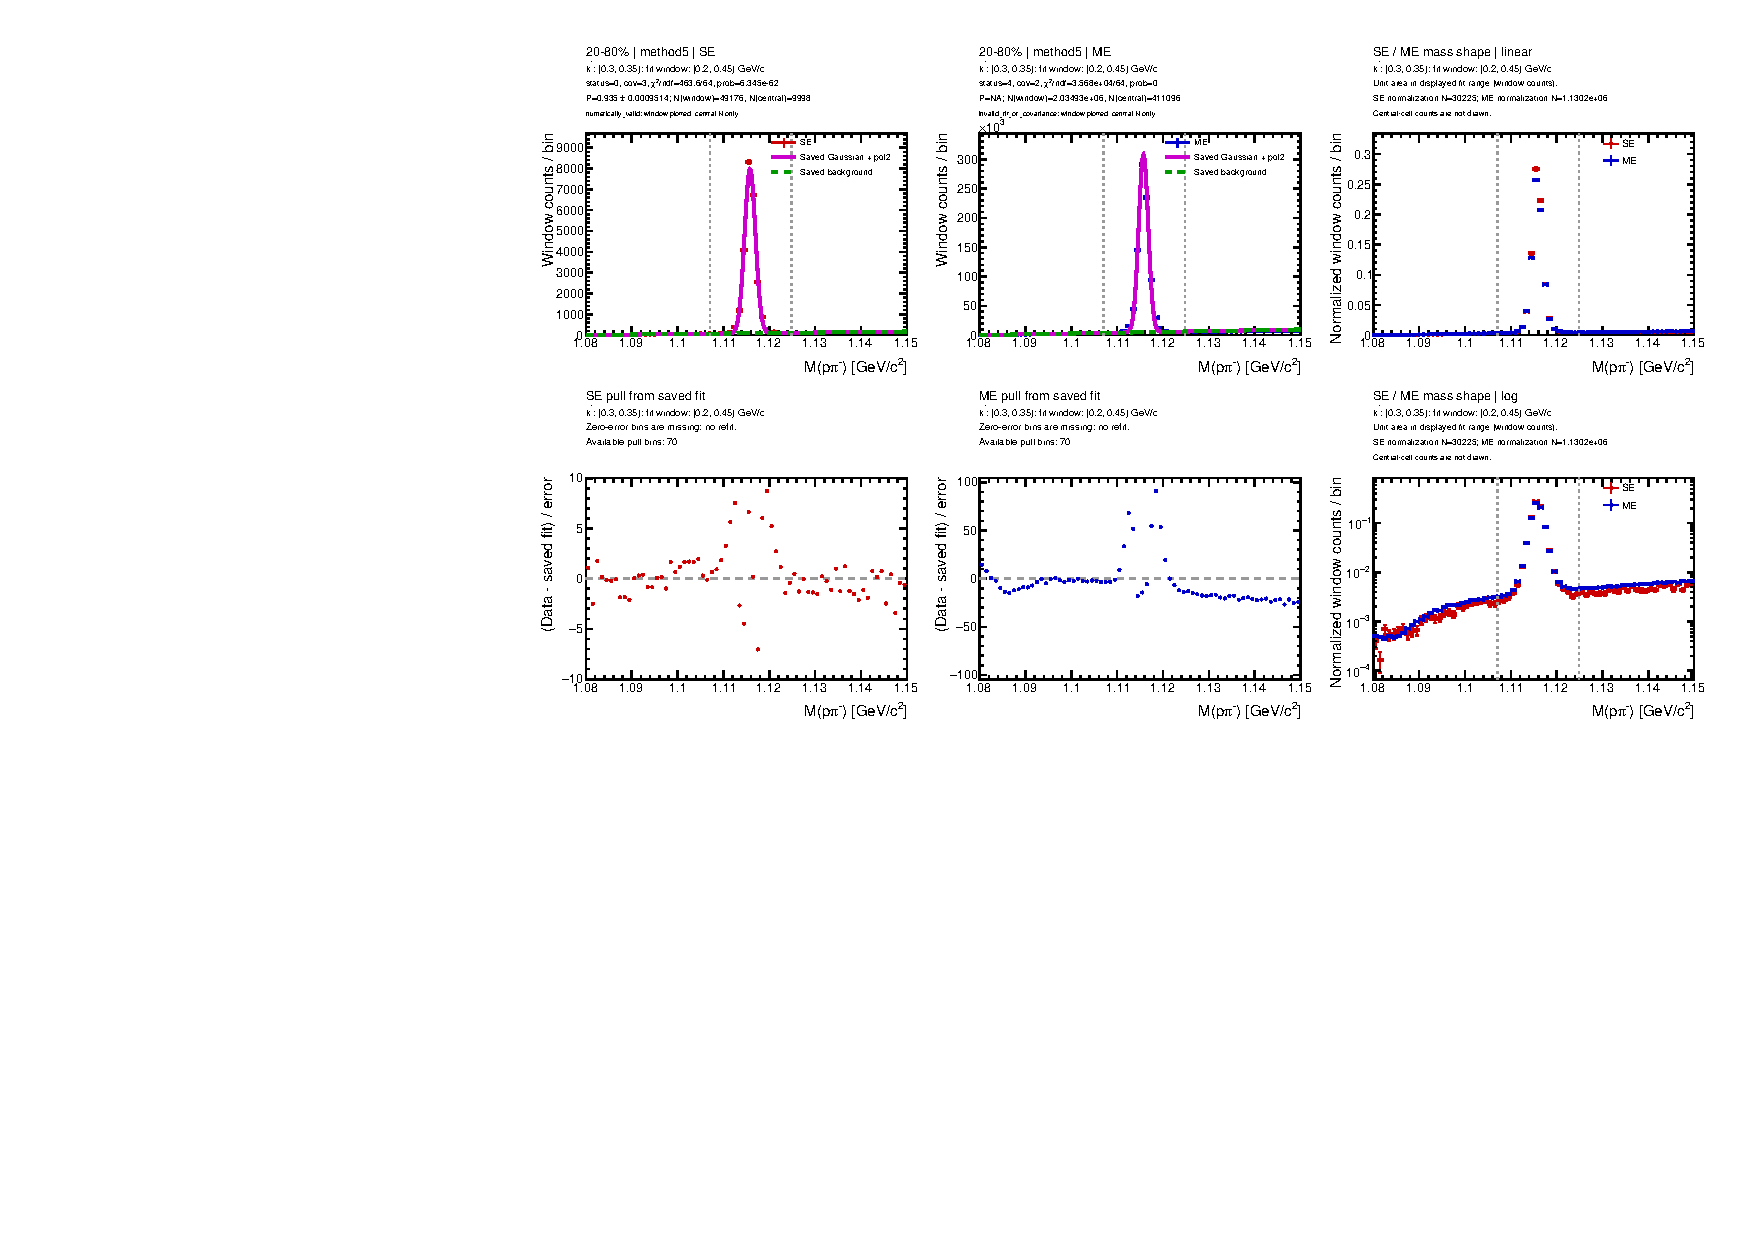
\includepdf[pages={1},fitpaper=true,pagecommand={}]{fit_method5_cent20_80_007.pdf}
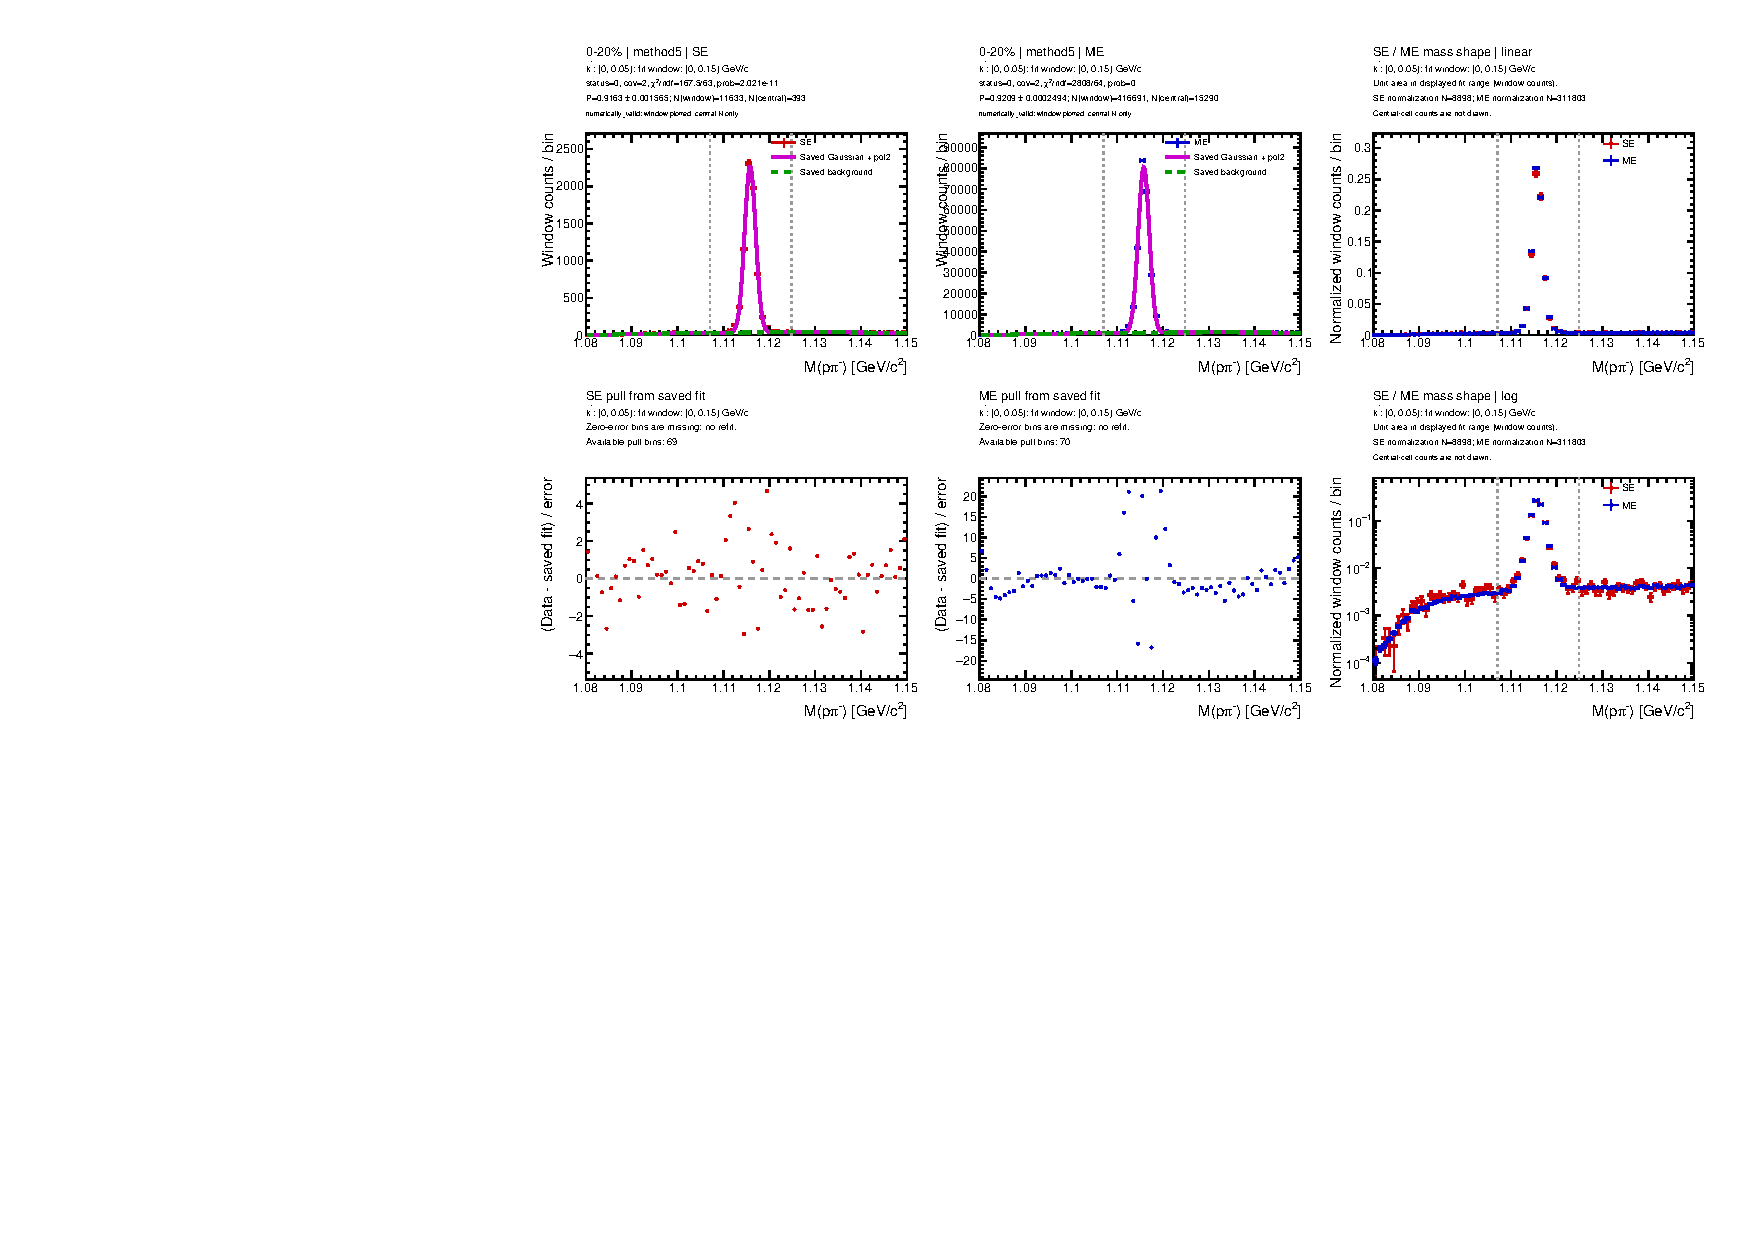
\includepdf[pages={1},fitpaper=true,pagecommand={}]{fit_method5_cent0_20_001.pdf}
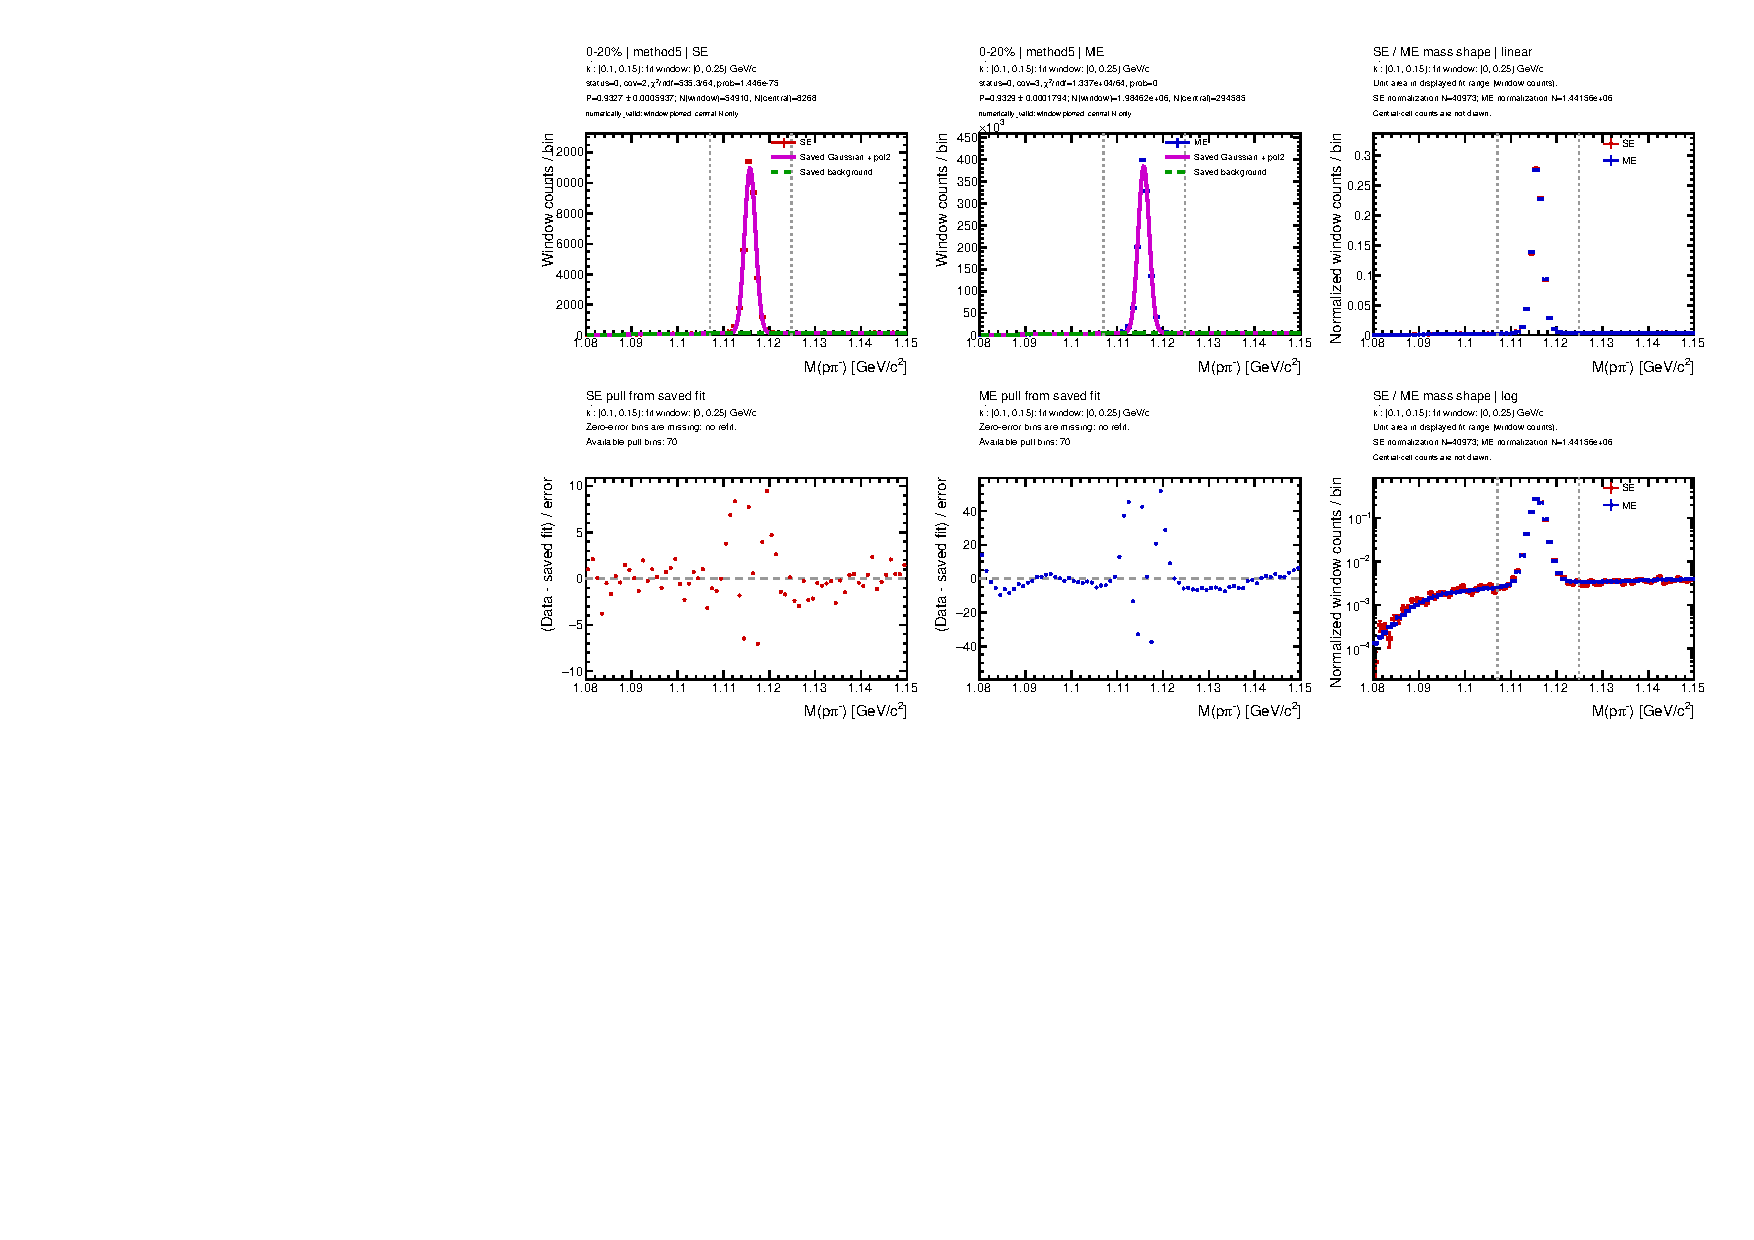
\includepdf[pages={1},fitpaper=true,pagecommand={}]{fit_method5_cent0_20_003.pdf}
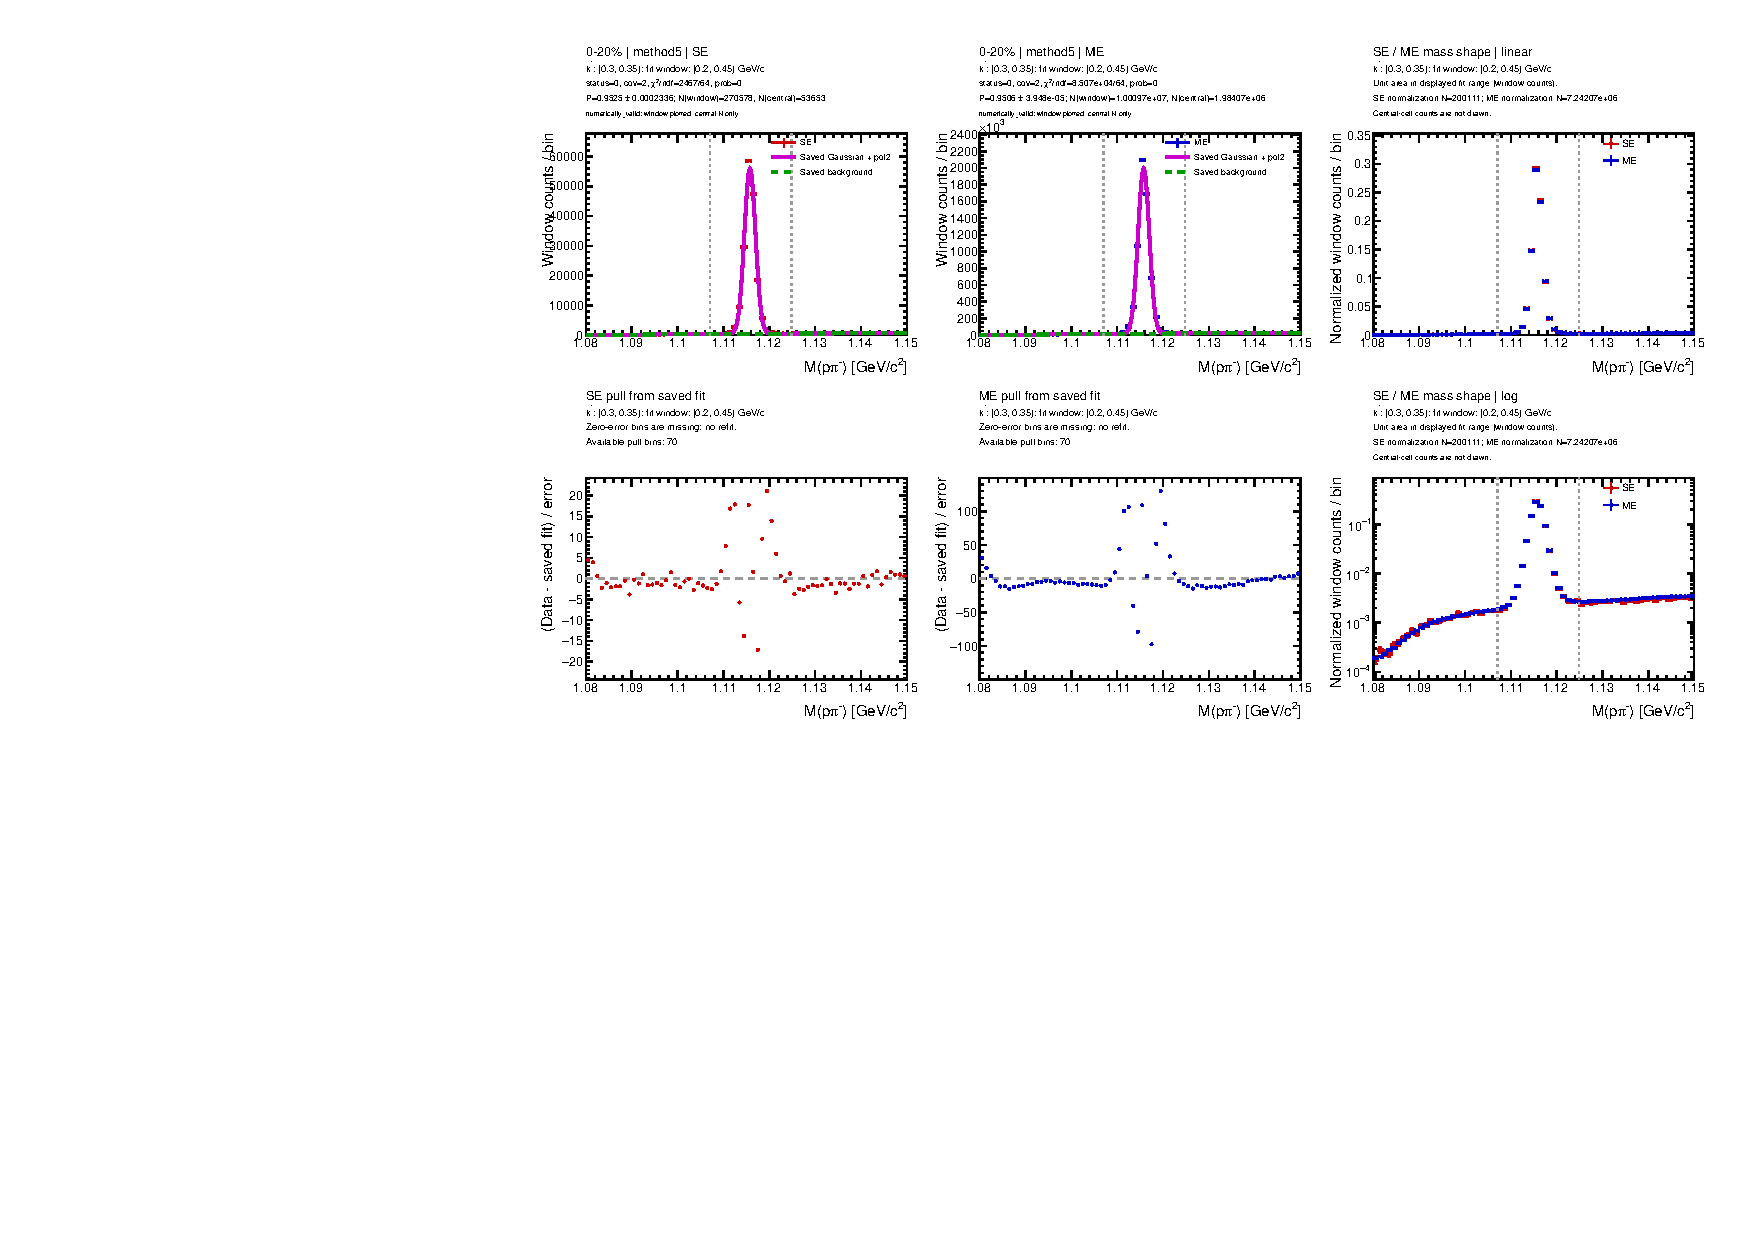
\includepdf[pages={1},fitpaper=true,pagecommand={}]{fit_method5_cent0_20_007.pdf}
\end{document}
